\chapter{Experiments} \label{chp:experiments}
\section{Suppression Task} \label{sec:sup}
\subsection{Intuitive Overview} \label{ssec:sup_intuition}
The Suppression Task refers to an experiment conducted by \cite{byrne1989suppressing} and is a classical example of the inadequacy of monotonic logics for modelling human reasoning. In classical logic, if our knowledge base $S$ is such that $I(S) \models \phi$, then it must be the case that $I(S \cup \psi) \models \phi$. However, in the suppression task participants no longer draw classically valid inferences when new information is added. The task is often formulated as follows:

\begin{itemize}
\item $(l|e)$: If she has an essay to write ($e$), she will study late in the library ($l$).
\item $(e \leftarrow \top)$: She has an essay to write ($e$).
\item $(l|o)$: If the library is open ($o$), she will study late in the library ($l$).
\end{itemize}

Given only the rule $e\leftarrow \top$ and conditional $(l|e)$, the participants consistently concluded that she would study late in the library, seemingly interpreting $(l|e)$ as $l\leftarrow e$ and drawing the classical logic inference $\frac{l \leftarrow e, e}{l}$ with \textit{modus ponens}. But when given the additional conditional $(l|o)$, participants no longer believe that they have enough information to judge whether she will study late in the library, and a significant portion of them no longer draw the classical conclusion. This effect, called Suppression, demonstrates the need for something more than classical logic for modelling human reasoning.

\subsection{Modelling the Suppression Task: WCS} \label{ssec:sup_mod}
Work by \cite{dietz2014modeling} has shown that the WCS is an adequate non-monotonic logic for modelling the Suppression Task. Under the WCS and \L ukasiewicz 3-valued logic the task is usually modelled using an epistemic knowledge base $\text{KB}_\text{noSup}$, with:
\[\text{KB}_\text{noSup}=(S=\{e \leftarrow \top\}, \Delta=\{(l|e)\})\]
Which represents the  task without the suppressing conditional $(l|o)$. Interpreting the conditional as a license for implication, as in Section~\ref{ssec:condInterpretation}, the knowledge base can be rewritten as a propositional knowledge base:
\[\text{KB}_\text{noSup}=\{e \leftarrow \top, l \leftarrow e \land \lnot \text{ab}_1, \text{ab}_1\leftarrow \bot\})\]
Weakly completing $\text{KB}_\text{noSup}$ results in:
\[\text{wc KB}_\text{noSup}=\{e \leftrightarrow \top, l \leftrightarrow e \land \lnot \text{ab}_1, \text{ab}_1\leftrightarrow \bot\}\]
Finally application of the semantic operator results in $\top=\{e\}, \bot=\{ab_1\}$ after the first execution and converges to the least model $\top=\{e,l\}, \bot=\{ab_1\}$.

After application of the semantic operator $l$ is true in the least model, and so participants conclude that she will study late in the library (as when $\text{KB}_\text{noSup}$ is evaluated classically). However, in the case where Suppression is observed, the same process yields a different result because of the presence of the extra conditional $(l|o)$.

Now the initial knowledge base $\text{KB}_\text{sup}$ includes the conditional $(l|o)$:
\[\text{KB}_\text{sup}=(S=\{e \leftarrow \top\}, \Delta=\{(l|e),(l|o)\})\]
And, when rewritten as a propositional knowledge base:
\[\text{KB}_\text{sup}=\{e \leftarrow \top, l \leftarrow e \land \lnot \text{ab}_1, l \leftarrow o \land \lnot \text{ab}_2, \text{ab}_1\leftarrow \lnot o, \text{ab}_2\leftarrow \lnot e\})\]
Where the abnormalities added to the interpretation of conditionals ($\psi|\text{body}$) which share $\psi$ as a head are considered dependent on one another. Weakly completing this knowledge base results in:
\[\text{WC KB}_\text{sup}=\{e \leftrightarrow \top, l \leftrightarrow (e \land \lnot \text{ab}_1) \land (o \land \lnot \text{ab}_2), \text{ab}_1\leftrightarrow \lnot o, \text{ab}_2\leftrightarrow \lnot e\})\]
For which applying the semantic operator converges to the least model $\top=\{e\},\bot=\{ab_2\}$ after the first application.

Now suppression has been displayed in the logic program and the variable $l$ remains unknown in the least model.

\subsection{Modelling the Suppression Task: Reiter's Default Logic}
\cite{ragni2017formal} showed that it was not possible to model the suppression task using Reiter's Default Logic. They created a default theory $(W, D'_P)$ as an illustration of Default Theory to illustrate this point.

A naive Default Theory for the suppression task $(W,D_\text{naive})$ can be used to model the classical logic response to the suppression task (i.e. that she will study late in the library), by treating the conditional as an implication without an associated abnormality predicate.
\[
W=\{e\leftarrow \top\}
\]
\[
D_\text{naive}=\{\delta_1:\frac{e\leftarrow \top:l \leftarrow \bot}{l\leftarrow\top} ,
\}
\]
\[
D'_\text{naive}=\{\delta_1:\frac{e\leftarrow \top:l \leftarrow \bot}{l\leftarrow\top} ,
\{\delta_2:\frac{o\leftarrow \top:l \leftarrow \bot}{l\leftarrow\top}
\}
\]
The only closed and successful default process that can generated for this task is $\Pi_\text{naive}=(\delta_1)$, which results in the inset $\text{In}(\Pi_\text{naive})=\{e\leftarrow \top, l\leftarrow\top\}$. When the set of default rules is extended to create $D'_\text{naive}$ which describes information about if the library is open, then the inset $\text{In}(\Pi_\text{naive})=\{e\leftarrow \top, l\leftarrow\top\}$, and $\{\delta_1\}$ remains the only extension. Both theories assert that she will study late in the library and suppression is not observed.

Even generalising our WCS approach to the Suppression Task and defining a set of defaults $D_P$ which capture intuition about abnormalities, fails to demonstrate suppression.
\[
D_P=\{\delta_1:\frac{e\leftarrow \top:\text{ab}_1 \leftarrow \bot}{l\leftarrow\top} ,
\delta_2:\frac{:\text{ab}_1 \leftarrow \top}{\text{ab}_1\leftarrow\top}
\}
\]
\[
D'_P=\{\delta_1:\frac{e\leftarrow \top:\text{ab}_1 \leftarrow \bot}{l\leftarrow\top} ,
\delta_2:\frac{o\leftarrow \top:\text{ab}_2 \leftarrow \bot}{l\leftarrow\top},
\delta_3:\frac{o\leftarrow \bot:\text{ab}_1 \leftarrow \top}{\text{ab}_1\leftarrow\top},
\delta_4:\frac{e\leftarrow \bot:\text{ab}_2 \leftarrow \top}{\text{ab}_2\leftarrow\top}
\}
\]

For the theory $(W,D_P)$, the only closed and successful default processes which produce extensions are $\Pi_P^1=(\delta_1,\delta_2)$ and $\Pi^2_P=(\delta_2,\delta_1)$, with $(l\leftarrow \top)\in \text{In}(\Pi^1_P)$ and $(l\leftarrow \top)\in \text{In}(\Pi^2_P)$. For the theory $(W,D'_P)$ the only closed and successful default process is $\Pi'_P=(\delta_1)$ and $(l\leftarrow \top)\in \text{In}(\Pi'_P)$, thus neither theory demonstrates suppression.

\section{Wason Selection Task}
\begin{table}
\begin{center}


\begin{tabular}{ c c c c c}
  & \textbf{$D$} & \textbf{$Dn3$} & \textbf{$Dn3n7$} & \textbf{$Dn7$}\\ 
  \hline
 Abstract & 36 & 39 & 5 & 19\\  
\end{tabular}
\caption{The canonical results of the Wason Selection Task for the Abstract case.}
\label{tbl:can}
\end{center}
\end{table}

\begin{table}
\begin{center}
\begin{tabular}{ c c c c c}
  & \textbf{$p$} & \textbf{$pq$} & \textbf{$pq\bar{q}$} & \textbf{$p\bar{q}$}\\ 
  \hline
 Abstract & 36 & 39 & 5 & 19\\  
 Everyday & 23 & 37 & 11 & 29\\  
 Deontic & 13 & 19 & 4 & 64
\end{tabular}
\caption{The canonical results of the Wason Selection Task over the Abstract, Everyday, and Deontic Cases}
\label{tbl:can_full}
\end{center}
\end{table}

Another widely studied task in the psychological literature is the Wason Selection Task (WST), which asks participants to draw conclusions about which variables are able to falsify a given rule (\textit{Modus Tolens}\footnote{If $a\rightarrow b$, then $\lnot b \rightarrow \lnot a$}). The task has many formulations (including the Abstract, Everyday, and Deontic cases), but this thesis will exam one of the most mostly widely researched cases: the Abstract case. 

\begin{figure}
\begin{center}
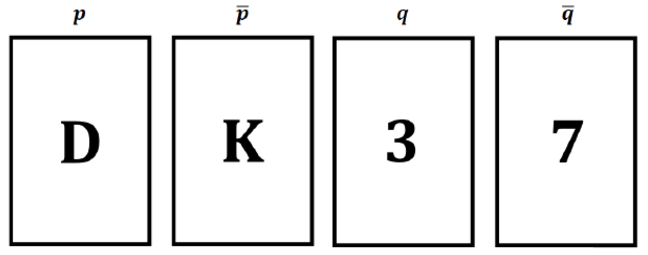
\includegraphics[scale=0.5]{wasonAbstract}
\caption{The Abstract case of the Wason Selection Task}
\label{fig:wst}
\end{center}

\end{figure}

The Abstract case of the WST presents the subject with four cards on a table as shown in Figure~\ref{fig:wst}. Their face-up sides read $D, K, 3,$ and $7$. Participants are told that each card has a number on one side and a letter on the other. They are then asked which cards must be turned over to test the rule:

\begin{center}
``If there is a $D$ on one side of the card, then the other side shows $3$."
\end{center} 

\begin{table}
\begin{center}


\begin{tabular}{ c c c}
  \textbf{$D$}&  \textbf{$3$}& \textbf{$3\leftarrow D$} \\ 
  \hline
 $\top$ & $\top$ & $\top$\\  
 $\top$ & $\bot$ & $\bot$\\  
 $\bot$ & $\top$ & $\top$\\
 $\bot$ & $\bot$ & $\top$
\end{tabular}
\caption{Propositional evaluation of the implication $3 \leftarrow D$ for each possible truth value of $3$ and $D$.}
\label{tbl:wst_impl}
\end{center}
\end{table}

\begin{table}
\begin{center}


\begin{tabular}{ c c c}
  \textbf{$D$}&  \textbf{$3$}& \textbf{$(3|D)$} \\ 
  \hline
 $\top$ & $\top$ & verification\\  
  $\top$ & $u$ & non-applicability\\ 
 $\top$ & $\bot$ & falsification\\  
 $\bot$ & $\cdot$ & non-applicability\\
 $u$ & $\cdot$ & non-applicability
\end{tabular}
\caption{De-finetti evaluation of the conditional $(3|D)$ for each possible truth value of $3$ and $D$.}
\label{tbl:wst_classical}
\end{center}
\end{table}

\begin{figure}
\centering 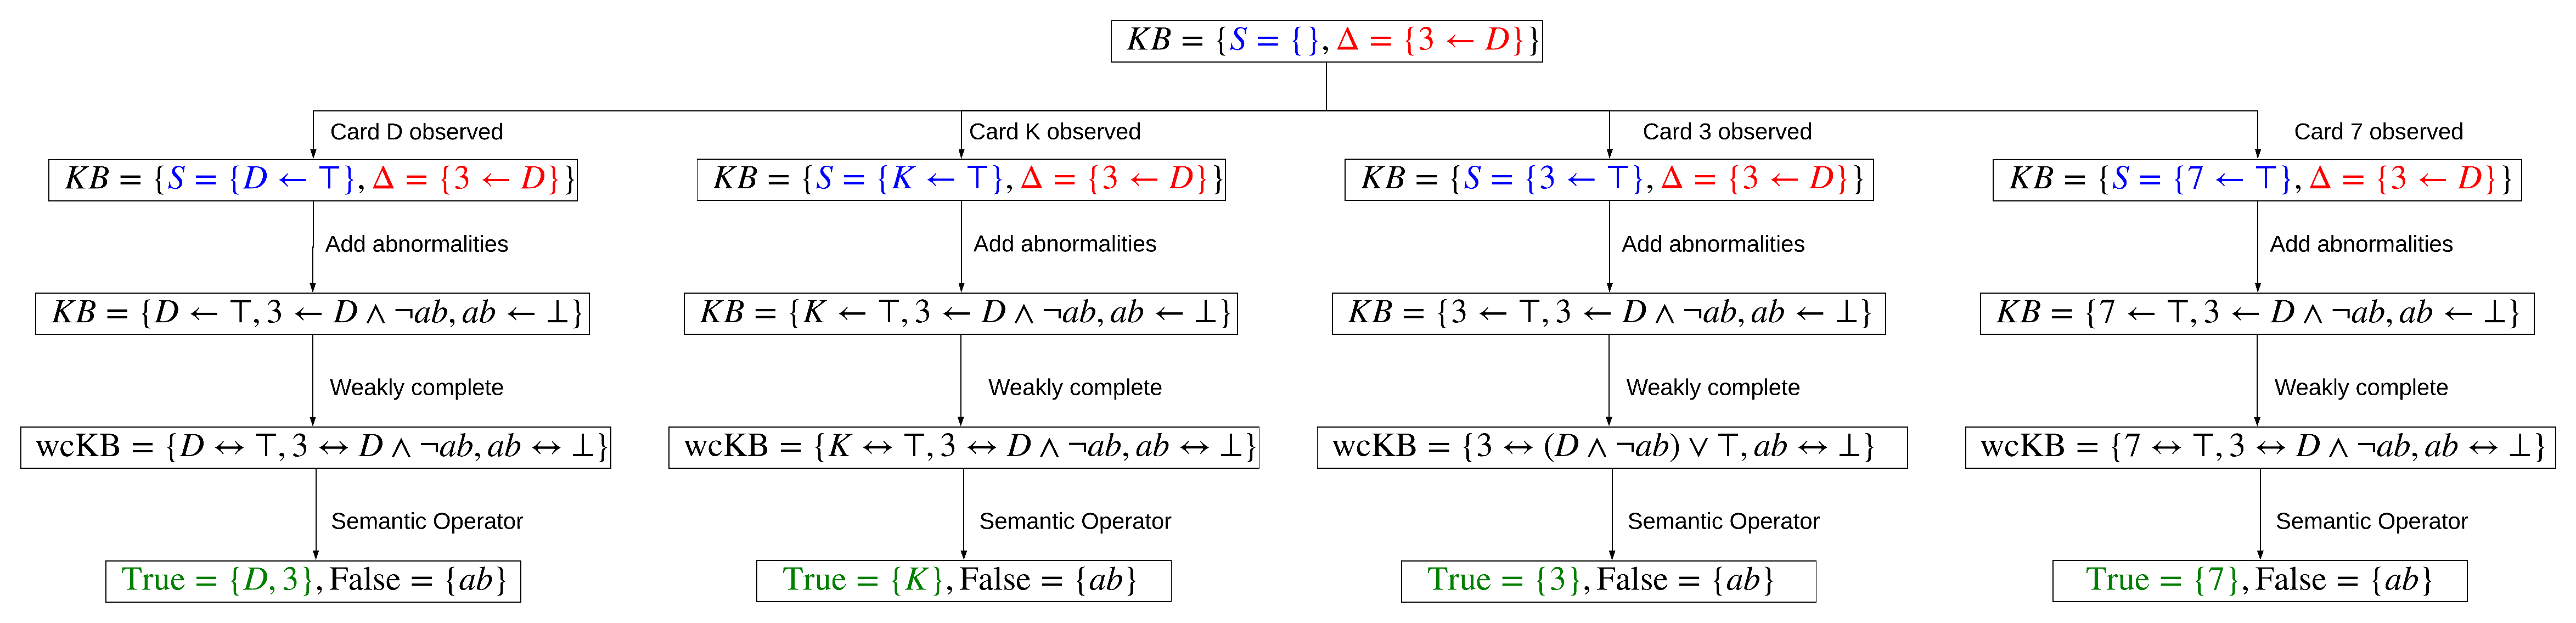
\includegraphics[scale=0.4]{WST_WCS}
\caption{Application of the WCS to the abstract case of the WST for the basic weak completion approach.}
\label{wst_wcs}
\end{figure}

This task requires the participants to find possible defeaters for the conditional rule. Assuming the \textit{de Finetti} truth table from Section~\ref{ssec:condi} for the interpretation of conditionals of the form ``If $\psi$ then $\phi$", Table~\ref{tbl:wst_impl} shows that the cards pairs $(D,3)$ and $(D,7)$ are both possible defeaters to the rule $(3 \leftarrow D)$ because the rule $(3|D)$ is only verified or falsified when the interpretation maps $(D,\top)$ and $(3, \lnot u)$. Any observed card which allows a possible world with both of those assignments is a possible defeater. If a participant were to turn the $D$ card and find a number that was not $3$, or were to a turn the card $7$ and find the letter $D$ on the other side, the classical interpretation of conditional would not hold. Thus these two cards must be turned to check the rule. However, human subjects very seldom choose this classical answer set and instead overwhelmingly prefer to turn the cards $D$ and $3$. Table~\ref{tbl:can} shows the most common card selection sets for participants.

A great many cognitive theories have been applied to these results, with varying degrees of success \citep{ragni2017formal}. This paper will focus on the WCS interpretation of the task provided by \cite{ragni2017wason}. This approach assumed an initial knowledge base $\text{KB}$ containing only the conditional $(3|D)$ and an interpretation of the conditional as a license for implication.

\cite{dietz2012computational} showed that the abstract case of the WST could be modelled using the WCS and 3-valued \L ukasiewicz logic. Using the conditional as the initial logic program, we write $KB=(S=\{\},\Delta=(3|D))$. Treating conditionals as licenses for implication $\text{KB}$ can be rewritten as $\text{KB}=(3\leftarrow D \land \lnot \text{ab}_1)$ where $\text{ab}_1$ is an abnormality predicate. Now $\textrm{lm wc}(KB)=\{\}\{ab\}$, and no information is obtained that could either verify or falsify the conditional. In order to adapt the WCS to the WST they introduced the concept of observation support.

\begin{table}
\begin{center}


\begin{tabular}{ c c c c }
  \textbf{Observation $O$}&  \textbf{Explanation $\epsilon$}&\textbf{$\text{lm wc (KB}\cup \epsilon)$}& \textbf{Turn Function} \\ 
  \hline
 $D$ & $\{D\leftarrow \top\}$ & $\{D,3\}\{\text{ab}_1\}$&turn\\  
 $K$ & $\{K\leftarrow \top\}$ & $\{K\}\{\text{ab}_1\}$&do not turn\\  
 $3$ & $\{D\leftarrow\top\}$ &$\{D,3\}\{\text{ab}_1\}$&turn\\
 $7$ & $\{7 \leftarrow \top\}$ & $\{7\}\{\text{ab}_1\}$&do not turn
\end{tabular}
\caption{Dietz' computational logic approach to the abstract case of the WST.}
\label{tbl:wst_lmwc}
\end{center}
\end{table}

The set of abducibles $A$ corresponds to positive and negative facts which are not assigned in $KB$. For the WST as formulated here $A=\{D\leftarrow \top,D\leftarrow \bot,3\leftarrow \top,3\leftarrow \bot,K\leftarrow \top,K\leftarrow \bot,7\leftarrow \top,7\leftarrow \bot\}$.
 An observation $O$ is explained by a minimal explanation $\epsilon \in A$ if and only if $O$ holds in $\textrm{lm wc}(KB\cup\epsilon)$. Table~\ref{tbl:wst_lmwc} shows the least models that can be drawn for the observations $D$, $3$, $K$, and $7$. If a least model obtained in this way contains atoms and atomic assignments that could verify or falsify the conditional (i.e. make $I_{\textrm{lm wc}(KB\cup \epsilon)}(3|D)\neq$ non-applicability), then the observed card should be turned. Figure~\ref{wst_wcs} shows the derivation of $\textrm{lm wc}(KB\cup \epsilon)$ for $\epsilon=D, \epsilon=3, \epsilon=K$, and $\epsilon=7$.\footnote{This approach differs in description from the author's original one, in which a card was turned if the least model assigned non-$u$ values to every variable in the conditional (i.e. $3$ and $D$), but is identical in practice.}


This simple interpretation of the WST which applies abduction to the initial knowledge base to derive observation is sufficient to model the general reasoner. It does not however explain any of the other deviant cases which are observed in Table~\ref{tbl:can}. Why, for example, should it be considered accurate if it gives no information about the classically accurate choice of the $D$ and $7$ cards, chosen by 19 participants, a significant proportion? Instead, consider how these aberrant reasoners could be modelled. Perhaps they use extra computational steps or omit steps? This author has previously shown that the WCS is able to model these individual reasoners \citep{breu2019weak}\footnote{My contribution to this paper was the initial proposal of the extensions, their integration, the silencing mechanism used for modelling individual reasoners, and the broad idea of the stochastic evaluation technique itself.} by including three simple processes: \textit{basic weak completion}, \textit{abduction} (as we have already discussed in this section), and \textit{contraposition}. By including these three processes, and stochastically controlling when they are activated or silenced, it has been shown that not only is this extended framework able to model the major cases of the WCS, but very close approximations to empirical frequency results can also be drawn for all three cases of the WST (Table~\ref{tbl:can_full}).

\subsubsection*{Basic Weak Completion}

Basic weak completion ignores the existence of other least models which may validate or invalidate the inference $(3|D)$ and, instead handles only those cases where $\epsilon \leftrightarrow (O\leftarrow \top)$. That is, only information about the currently observed card is considered in the abductive framework. Figure~\ref{wst_wcs} illustrates this process for each of the four observations: $D$, $3$, $K$, and $7$. Now only $\textrm{wc lm}(KB \cup (D \leftarrow \top))$ provides assignments which for which the de Finetti interpretation of $(3|D)\neq \textrm{non-applicability}$. Observing the card $3$ no longer leads to the decision to turn the card because only the case $\epsilon = (3\leftarrow \top)$ is considered and the case $\epsilon = (D \leftarrow \top)$ is not considered.

\subsubsection*{Contraposition}
\begin{table}
\begin{center}
\begin{tabular}{ c c c }
 \textbf{Iteration} & \textbf{$\top$} & \textbf{$\bot$} \\ 
 \hline
 0 &  &  \\  
 1 &  $7$ & $ab_1$, $ab_2$  \\  
 2 &  $7$ & $3$, $ab_1$, $ab_2$  \\
 3 &  $7$, $D'$ & $3$, $ab_1$, $ab_2$  \\
 4 &  $7$, $D'$ & $3$, $ab_1$, $ab_2$, $D$  
\end{tabular}
\caption{Applying the Weak Completion Semantics and Contraposition to the $7$ card of the WST.}
\label{tbl:7cont}
\end{center}
\end{table}

Contraposition implicitly makes use of \textit{modus tolens}, usually assumed to be silenced in human cognition, to derive certain canonical cases in the WST. Using contraposition it becomes possible to model individual participants who choose to turn the cards $D$ and $7$ (the classical response).

Contraposition is applied as follows for the initial knowledge base $KB$:
\begin{enumerate}
\item For each conditional $(\psi|\phi)\in KB'$ :
\begin{itemize}
\item Add the conditional $(\phi'|X)$ to $\Delta$, where $X$ is the other possible value for that card face\footnote{$(D,K),(3,7)$}.
\item Add the fact $\phi\leftarrow \lnot \phi'$ to $S$.
\end{itemize}
\item Interpret conditionals as licenses for implication.
\item Apply the Abductive case of the WCS as normal.
\item Turn the card if and only if some or $I_{\text{lm WC (KB} \cup \epsilon)}(\psi|\phi)\neq\textrm{non-applicability}$ or some $I_{\text{lm WC (KB} \cup \epsilon)}(\phi'|X)\neq\textrm{non-applicability}$, and $text{lm WC (KB} \cup \epsilon)$ explains $O$.
\end{enumerate}

Using this technique, and applying basic weak completion (i.e. only considering the case $\epsilon\leftrightarrow(O\leftarrow \top)$ it is possible to model the classical case of the WST. The resolution for the $7$ card is as follows:

\[
KB = (S=\{\},\Delta=\{(3|D)\})
\]
\[
KB' = (S=\{D \leftarrow  \lnot D'\},\Delta\{=(3|D),(D'|7)\})
\]
\[
KB' = \{3 \leftarrow D \land \lnot \text{ab}_1, D' \leftarrow 7 \land \lnot \text{ab}_2, \text{ab}_1 \leftarrow \bot, \text{ab}_2 \leftarrow \bot\}\}
\]
\[
KB'\cup (7\leftarrow\top) = \{3 \leftarrow D \land \lnot \text{ab}_1, D' \leftarrow 7 \land \lnot \text{ab}_2, \text{ab}_1 \leftarrow \bot, \text{ab}_2 \leftarrow \bot, 7 \leftarrow \top\}\}
\]
\[
\text{wc}KB'\cup (7\leftarrow\top) = \{3 \leftrightarrow D \land \lnot \text{ab}_1, D' \leftrightarrow 7 \land \lnot \text{ab}_2, \text{ab}_1 \leftrightarrow \bot, \text{ab}_2 \leftrightarrow \bot, 7 \leftrightarrow \top\}\}
\]
\begin{equation} \label{eqn:wst_contra}
\textrm{wc} (KB'\cup (7\leftarrow\top)) = \{3 \leftrightarrow D \land \lnot ab_1, D' \leftrightarrow (\lnot 3 \land ab_2) \lor (\lnot D),  ab_2\leftrightarrow \bot, ab_1\leftrightarrow \bot, 7\leftrightarrow\top \}
\end{equation}

Table~\ref{tbl:7cont} shows the computation of $\textrm{lm wc} (KB'\cup (7\leftarrow\top))$. From this, it is possible to deduce that the card $7$ must be turned. Figure~\ref{fig:wstcano} illustrates the use of these extensions to derive all four of the canonical cases of the WST.

 
\subsubsection*{Combined Model}
By combining our contraposition and abductive models for inferences, it is possible to model the case where the cards $D$, $3$, and $7$ are turned. Combining the models $(A_i,...,A_n)$ is done by turning a card $c$ if and only if $c$ would be turned in some model $A_i$.

This work has shown that all canonical cases of the weak completion semantics can be modelled by activating or silencing these three processes on the initial knowledge base. The intuition that a discrete and systematic succession of well-founded processes could be used to model multiple different results for the same experiment was the inspiration for the SCP framework which this thesis introduces.


\begin{figure}
\centering 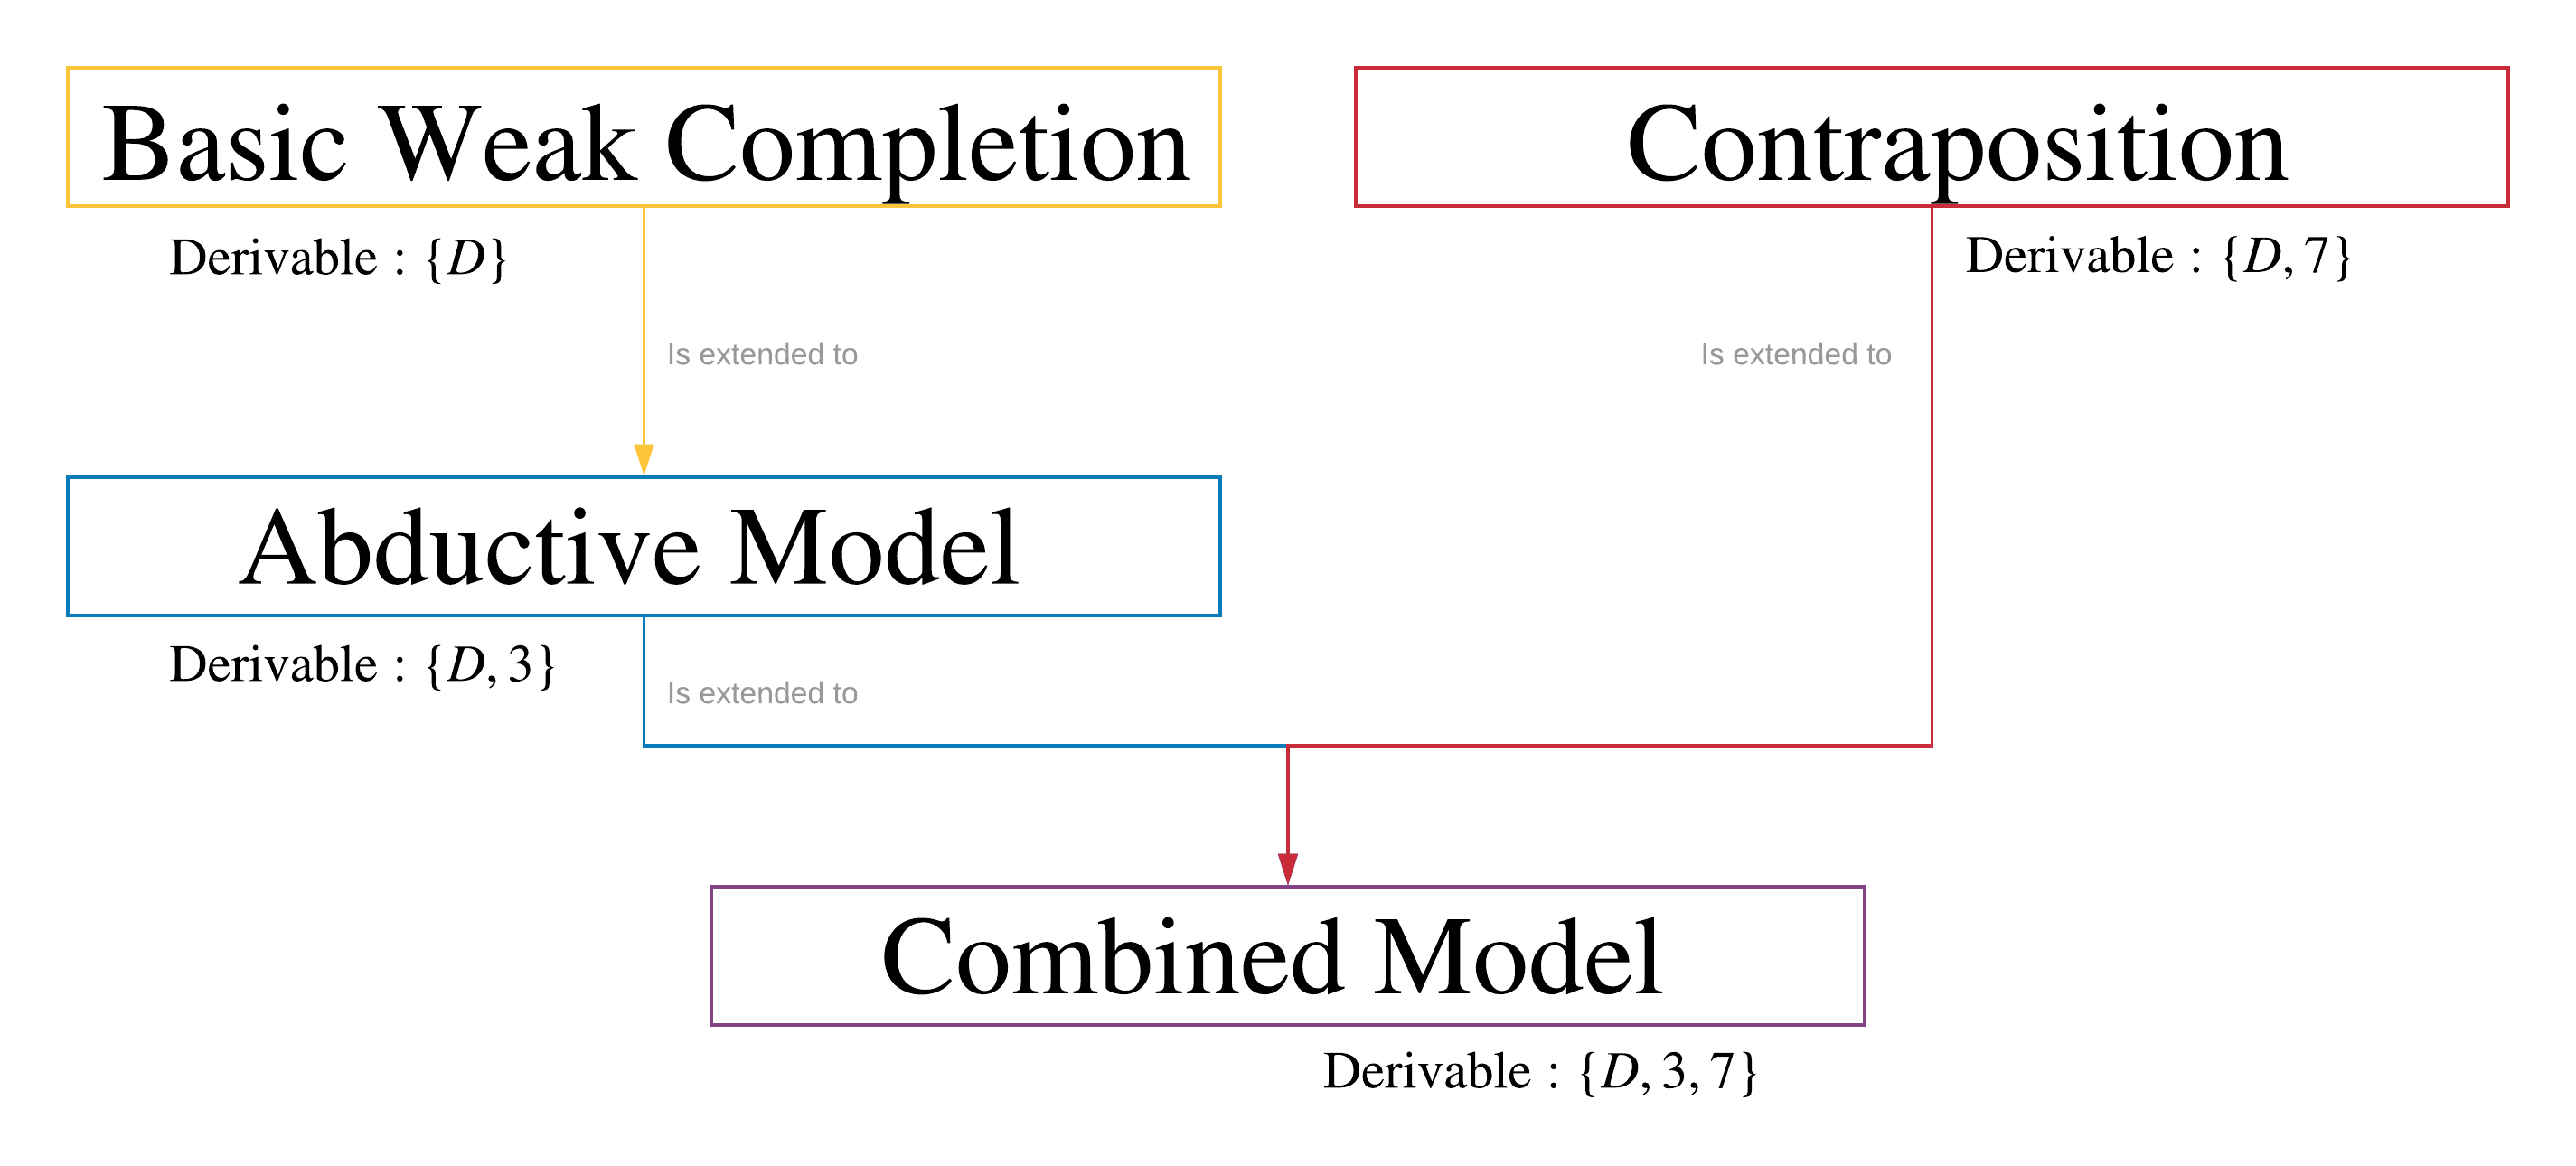
\includegraphics[scale=.6]{wst_cano}
\caption{Using the abduction and contraposition extensions to derive all four canonical cases. Arrows indicate that the origin model produces a subset of the turn instructions of the endpoint.}
\label{fig:wstcano}
\end{figure}




















